%!LW recipe=pdflatex

\documentclass[12pt,aspectratio=169]{beamer}
% \hypersetup{pdfpagemode=FullScreen}

\usepackage{upgreek}
\usefonttheme{professionalfonts}
\usepackage{mathtools}

\renewcommand*{\thefootnote}{\fnsymbol{footnote}}

\DeclareUnicodeCharacter{0301}{\'{e}}

\makeatletter
\def\onlyfootnote{\gdef\@thefnmark{}\@footnotetext}
\makeatother

\mode<presentation>
\useoutertheme[subsection=false]{miniframes}

\AtBeginSection[]{
    \begin{frame}
    \centering
    \begin{beamercolorbox}[sep=8pt,center,shadow=true,rounded=true]{title}
        \usebeamerfont{title}\insertsectionhead\par%
    \end{beamercolorbox}
    \end{frame}
}

\title{Retrieval-Augmented Generation for Knowledge-Intensive NLP Tasks}
\author{ \small
    Patrick~Lewis\inst{1,2}\and
    Ethan~Perez\inst{3}\and
    Aleksandra~Piktus\inst{1}\and
    Fabio~Petroni\inst{1}\and
    Vladimir~Karpukhin\inst{1}\and
    Naman~Goyal\inst{1}\and
    Heinrich~Küttler\inst{1}\and
    Mike~Lewis\inst{1}\and
    Wen-tau~Yih\inst{1}\and
    Tim~Rocktäschel\inst{1,2}\and
    Sebastian~Riedel\inst{1,2}\and
    Douwe~Kiela\inst{1}
}
\institute{
    \inst{1}Facebook AI Research \\
    \inst{2}University College London \\
    \inst{3}New York University
}
\date{Presenter: Shiwei Zhang}

\begin{document}
    \beamertemplatenavigationsymbolsempty

    \begin{frame}[plain]
        \titlepage
    \end{frame}

    \begin{frame}[plain]
        \centering
        \includegraphics[page=15,trim=53.99bp 410.30bp 42.33bp 53.63bp,clip,scale=0.75]{survey.pdf}
    \end{frame}

    \section*{Content}

    \begin{frame}
        \frametitle{Content}

        \begin{itemize}
            \setlength{\itemsep}{.8em}
            \item Introduction
            \item Models
            \item Training and Inference
            \item Experiments
            \item Conclusion
        \end{itemize}
    \end{frame}


    \section{Introduction}

    \begin{frame}
        \frametitle{Motivation}

        Pre-trained neural language models generate content based on parameterized implicit knowledge base. Such models
        have several downsides:

        \vskip .5em
        \begin{itemize}
            \setlength{\itemsep}{.4em}
            \item They cannot easily expand or revise their memory.
            \item They cannot straightforwardly provide insights into the predictions.
            \item They may produce ``hallucinations''.
        \end{itemize}
        \vskip .5em

        Hybrid models that combine parametric memory with non-parametric (i.e. retrieval-based) memories may address
        these issues.
    \end{frame}

    \begin{frame}
        \frametitle{Overview}

        Retriever $p_\eta(z|x)$ returns (top-K) probabilities over documents for query $x$.
        \vskip .5em
        Generator $p_\theta(y_i|x,z,y_{1:i-1})$ generates a current token based on a context of the previous $i-1$
        tokens $y_{1:i-1}$, the original input $x$, and a retrieved passage $z$.

        \vskip 1em
        \centering
        \includegraphics[page=2,trim=108.28bp 604.69bp 107.98bp 70.46bp,clip,scale=.9]{paper.pdf}
    \end{frame}


    \section{Models}

    \begin{frame}
        \frametitle{Marginalization}

        RAG treats the retrieved document as a latent variable and proposes two models to marginalize over the latent
        documents in different ways to produce a distribution over generated text.

        \vskip 1em
        \centering
        \large
        \[
        \begin{rcases*}
            p_\eta(z|x) \\
            p_\theta(y_i|x,z,y_{1:i-1})
        \end{rcases*} \overset{?}{\Rightarrow} p(y|x)
        \]

    \end{frame}

    \begin{frame}
        \frametitle{RAG-Sequence Model}

        The RAG-Sequence model uses the same retrieved document to generate the complete sequence.

        \begin{align*}
            p_{\text{\tiny RAG-Sequence}}(y|x) &\approx \sum_{z \in \operatorname*{top-k}(p(\cdot|x))} p_\eta(z|x)p_\theta(y|x,z)  \\
            & =\sum_{z\in\operatorname*{top-k}(p(\cdot|x))} p_\eta(z|x) \prod_i^N p_\theta(y_i|x,z,y_{1:i-1})
        \end{align*}
    \end{frame}

    \begin{frame}
        \frametitle{RAG-Token Model}

        The RAG-Token model draws a different latent document for each target token. This allows the generator to choose
        content from several documents when producing an answer.

        $$ p_{\text{\tiny RAG-Token}}(y|x) \approx \prod_i^N \sum_{z\in\operatorname*{top-k}(p(\cdot|x))} p_\eta(z|x)p_\theta(y_i|x,z_i,y_{1:i-1}) $$
    \end{frame}

    \begin{frame}
        \frametitle{Retriever: DPR}

        $$ p_\eta(z|x) \propto \exp(\mathbf{d}(z)^T\mathbf{q}(x)) \qquad \mathbf{d}(z) = \text{BERT}_d(z),\ \mathbf{q}(x) = \text{BERT}_q(x) $$

        \vskip .5em
        $\mathbf{d}(z)$ is a vector representation of a document produced by a BERT model and $\mathbf{q}(x)$ is a vector
        representation of the query produced by another BERT model.

        Calculating $\operatorname*{top-k}(p_\eta(\cdot|x))$ is a Maximum Inner Product Search (MIPS) problem, which can
        be approximately solved in sub-linear time.
    \end{frame}

    \begin{frame}
        \frametitle{Generator: BART}

        BART is a seq2seq transformer model with 400M parameters. RAG concatenates the input $x$ and the retrieved
        document $z$ to produce the input for BART.
    \end{frame}


    \section{Training and Inference}

    \begin{frame}
        \frametitle{Training}

        Given a fine-tuning training corpus of input/output pairs $(x_j, y_j)$, the retriever and generator are jointly
        trained by minimizing the negative marginal log-likelihood $\sum_j-\log p(y_j|x_j)$.

        \vskip 1em
        The document encoder $\text{BERT}_d$ is not updated during training as it is costly to do so (the document
        index needs to be updated as the model changes).
    \end{frame}

    \begin{frame}
        \frametitle{Decoding - RAG-Token}

        The RAG-Token model can be seen as a standard autoregressive seq2seq generator with transition probability:

        $$ p^\prime_\theta(y_i|x,y_{i:i-1}) = \sum_{z\in\operatorname*{top-k}(p(\cdot|x))}p_\eta(z_i|x)p_\theta(y_i|x,z_i,y_{1:i-1}) $$

        Standard beam-search decoder can be used to sample the output.
    \end{frame}

    \begin{frame}
        \frametitle{Decoding - RAG-Sequence}

        For RAG-Sequence, RAG runs beam search for each document $z$, scoring each hypothesis using
        $p_\theta(y_i|x,z,y_{1:i-1})$ and yielding a set of hypotheses $Y$. Some of the hypotheses may not appear in
        the beams of all documents.
        \vskip 1em
        If a hypothesis $y$ does not appear in a beam with document $z$, there are two options. The first option is to
        run an additional forward pass to get $p_\theta(y_i|x,z,y_{1:i-1})$. This is refered to as ``Thorough
        Decoding''. The other option is to assume $p_\theta(y|x,z_i) \approx 0$ if $y$ was not generated during beam
        search for $x,z_i$. This is refered to as ``Fast Decoding''.
    \end{frame}


    \section{Experiments}

    \begin{frame}
        \frametitle{Setup}

        \begin{itemize}
            \setlength{\itemsep}{.8em}
            \item \textbf{Non-parametric knowledge}: Dec. 2018 Wikipedia dump split into 100 word chunks, totaling 21M documents.
            \item \textbf{MIPS solver}: FAISS with Hierarchical Navigable Small World approximation.
            \item \textbf{Hyper-parameters}: $k \in \{5, 10\}$ when retrieving the top-k documents.
        \end{itemize}
    \end{frame}

    \begin{frame}
        \frametitle{Open-domain Question Answering}

        The four columns corresponds to four datasets.

        {
            \vskip 1em
            \centering
            \includegraphics[page=6,trim=107.66bp 576.05bp 310.33bp 124.59bp,clip]{paper.pdf}
            \vskip 1em
        }

        RAG can generate correct answers even if it is not in any retrieved document, where extractive models would score 0\%.

    \end{frame}

    \begin{frame}
        \frametitle{Abstractive Question Answering}

        This task consists of questions, ten gold passages retrieved from a search engine for each question, and a
        full sentence answer annotated from the retrieved passages.
        \vskip 1em
        RAG does not use the gold passages and relies only
        on its parametric and non-parametric (Wikipedia) knowledges.

        \vskip 1em
        \centering
        \includegraphics[page=6,trim=311.05bp 576.01bp 108.52bp 132.55bp,clip]{paper.pdf}
    \end{frame}

    \begin{frame}
        \frametitle{Jeopardy Question Generation}

        Jeopardy is about guessing an entity from a fact about that entity.

        {
            \vskip 1em
            \centering
            \includegraphics[page=6,trim=311.05bp 576.01bp 108.52bp 132.55bp,clip]{paper.pdf}
            \vskip 1em
        }

        Jeopardy questions often contain two separate pieces of information, and RAG-Token may perform
        best because it can generate responses that combine content from several documents.
    \end{frame}

    \begin{frame}
        \frametitle{Fact Verification}

        This task requires classifying a claim is supported or reduted by Wikipedia, or whether there is not enough
        information.

        \vskip 1em
        \centering
        \includegraphics[page=6,trim=311.05bp 576.01bp 108.52bp 132.55bp,clip]{paper.pdf}
    \end{frame}


    \section{Conclusion}

    \begin{frame}
        \frametitle{Conclusion}

        Strength:

        \begin{itemize}
            \setlength{\itemsep}{.4em}
            \item Addresses important problems.
            \item General and relatively simple formulation.
        \end{itemize}

        \vskip 1em
        Limitation (and Oppotunities):

        \begin{itemize}
            \setlength{\itemsep}{.4em}
            \item Does not actually solve the hallucination problem.
            \item Needs to run $k$ times more inference passes during generation.
            \item The input $x$ needs to be additionally processed by another model.
            \item The retrieving process is likely to be disk-IO intensive or memory demanding.
        \end{itemize}
    \end{frame}

    \appendix

    \begin{frame}
        \vskip 1em

        \centering \huge
        Thank you!
    \end{frame}
\end{document}
